\documentclass[12pt]{article}
\usepackage{packages}

\addbibresource{bibliography.bib}

\title{\vspace{-2.5em}Calculating the International Geomagnetic Reference Field}
\author{Björn Sundin}

\begin{document}

\maketitle

\section{Introduction}
The International Geomagnetic Reference Field (IGRF) is a three-dimensional model of Earth's internally generated magnetic field that is developed by the International Association of Geomagnetism and Aeronomy (IAGA) \parencite{Alken2021}. A new version is released every five years, because the process by which Earth's magnetic field is generated (magnetohydrodynamic dynamo) causes Earth's magnetic field to change over time.

In a region of space without currents or electromagnetic waves, the Ampère-Maxwell equation becomes $\nabla\crossproduct\vect{B} = 0$ and the field can be written as the negative gradient of a potential $V$; $\vect{B} = -\nabla V$. The IGRF model provides a list of spherical harmonic coeffients $g_n^m$ and $h_n^m$, which are used in the following equation to calculate the potential:
\begin{equation}
  V(r, \theta, \phi) = \sum_{n\,=\,0}^N\frac{a^{n+2}}{r^{n+1}}\sum_{m\,=\,0}^n\left(g_n^m\cos(m\phi) + h_n^m\sin(m\phi)\right)P_n^m(\cos\theta).
\end{equation}
Here $P_n^m(x)$ is the \textit{Schmidt semi-normalized associated Legendre function} of $n$th degree and $m$th order. The coefficients are in reality functions of time. The IGRF provides them at five-year intervals, and between these points they can be estimated via linear interpolation.

\section{Associated legendre functions}

The $n$th degree, $m$th order associated legendre function is defined as
\begin{equation}
  P_n^m(x) = \alpha_n^m(x)D^{m+n}(x^2-1)^n
\end{equation}
where
\begin{equation}
  \alpha_n^m(x) = \sqrt{(2-\delta_{m0})\frac{(n-m)!}{(n+m)!}}\frac{1}{2^nn!}(1-x^2)^{m/2},
\end{equation}
$\delta_{m0}$ is the Kronecker delta ($1$ for $m=0$ and $0$ otherwise) and $D = \derivative*{x}$ is the differentiation operator with respect to $x$.

\subsection{Expanded form}
The definition given above involves repeated differentiation, which is not very efficient to implement directly on a computer. The function $Q_n^m(x)=P_n^m(x)/\alpha_n^m(x)$ can be written as a polynomial by first expanding the binomial power:
\begin{equation}
  (x^2 - 1)^n = \displaystyle\sum_{k\,=\,0}^{n}{n\choose k}(-1)^{n-k}x^{2k}
\end{equation}
and then utilizing the following formula for repeated differentiation of a power function
\begin{equation}
  D^{n+m}x^{2k} = \begin{dcases}
    \frac{(2k)!}{(2k-n-m)!}x^{2k-n-m}, &\text{ if }m + n \leq 2k\\
    0, &\text{ if }m + n > 2k
  \end{dcases}.
\end{equation}
Both of these formulas can be proven by induction. Applying them, we get 
\begin{equation}
  Q_n^m(x) = D^{n+m}(x^2 - 1)^2 = \sum_{k\,=\,0}^{n}{n\choose k}(-1)^{n-k}\begin{dcases}
    \frac{(2k)!}{(2k-n-m)!}x^{2k-n-m}, &\text{ if }m + n \leq 2k\\
    0, &\text{ if }m + n > 2k
  \end{dcases}.
\end{equation}
Since
\begin{equation}
  m + n > 2k \Longleftrightarrow k < \frac{m+n}{2},
\end{equation}
all terms with $k<\ceil{(m+n)/2}$ are zero, and the equation can be simplified to
\begin{equation}
  Q_n^m(x) = \sum_{k\,=\,\ceil{(m+n)/2}}^{n}{n\choose k}\frac{(2k)!}{(2k-n-m)!}(-1)^{n-k}x^{2k-n-m}.
\end{equation}
This is more readily calculated, although it is still very computationally expensive, with a sum of multiple terms and five factorials to calculate per term. Something we can deduce though is that $Q_n^m(x)=0$ whenever $m+n>2n$, i.e. $m > n$. A faster way to calculate the $Q_n^m$s is to use recurrence relations, and the fact that $Q_n^m(x)=0$ for $m>n$ turns out to be important for doing that.

\subsection{Recurrence relations}
\begin{figure}[htbp]
  \centering
  \begin{tikzpicture}[>=stealth]
    \tikzmath{\N = 5;}

    \foreach \n in {0, ..., \N} {
      \foreach \m in {0, ..., \n} {
        \node (P\n\m) at (\m, -\n) {$P_{\n}^{\m}$};
      }
    }

    \pgfmathtruncatemacro{\Nminusone}{\N-1}
    \foreach \m in {0, ..., \Nminusone} {
      \foreach \n in {\m, ..., \Nminusone} {
        \pgfmathtruncatemacro{\next}{\n+1}
        \draw[->] (P\n\m) -- (P\next\m);
      }
    }

    \foreach \n in {0, ..., \Nminusone} {
      \pgfmathtruncatemacro{\next}{\n+1}
      \draw[->] (P\n\n) -- (P\next\next);
    }
  \end{tikzpicture}
  \caption{Diagram showing how the recurrence relations are used to calculate $P_n^m$.}
  \label{fig:recurrence-diagram}
\end{figure}

The idea is to 

\begin{figure}[htbp]
  \centering
  \begin{subfigure}{.49\linewidth}
    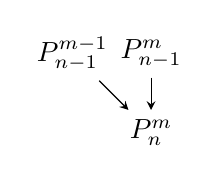
\begin{tikzpicture}[>=stealth]
      \node (Pnm) at (0, 0) {$P_{n}^{m}$};
      \node (Pn1m1) at (-1, 1) {$P_{n-1}^{m-1}$};
      \node (Pn1m) at (0, 1) {$P_{n-1}^{m}$};
      \draw[->] (Pn1m1) -- (Pnm);
      \draw[->] (Pn1m) -- (Pnm);
    \end{tikzpicture}
    \caption{}
  \end{subfigure}
  \begin{subfigure}{.49\linewidth}
    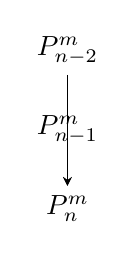
\begin{tikzpicture}[>=stealth]
      \node (Pnm) at (0, 0) {$P_{n}^{m}$};
      \node (Pn1m) at (0, 1) {$P_{n-1}^{m}$};
      \node (Pn2m) at (0, 2) {$P_{n-2}^{m}$};
      \draw[->] (Pn2m) -- (Pnm);
      \draw[->] (Pn1m) -- (Pnm);
    \end{tikzpicture}
    \caption{}
  \end{subfigure}
  \caption{Diagrams illustrating the two recurrence relations used.}
\end{figure}



% \begin{equation}
%   i = n - m + \begin{cases}
%     \displaystyle\sum_{k\,=\,0}^{m\,-\,1}(N-k), &\text{if }m\neq 0\\
%     0, &\text{if }m=0
%   \end{cases}
% \end{equation}
%
% \begin{equation}
%   \sum_{k\,=\,0}^{m\,-\,1}(N-k) = mN - \sum_{k\,=\,1}^{m\,-\,1}k = mN - \frac{(m-1)m}{2}
% \end{equation}

% \begin{equation}
%   P_n^m(x) = \frac{2n-1}{(n^2 - m^2)^{1/2}}x P_{n-1}^m(x) - \left(\frac{(n-1)^2 - m^2}{n^2 - m^2}\right)^{1/2}P_{n-2}^m(x)
% \end{equation}

\printbibliography

\end{document}
